\chapter{METHODOLOGY}
This chapter will explain the framework, game designs used, content, and evaluation form to evaluate the effectiveness and functionality of this project. The chapter will be divided into 4 parts: Content, System Design, Game Design, Evaluation Method.

\section{Content}
The content used in this project is taken from the class subject EGCI113 - Fundamental Programming. The content will start from simple topics such as type of variable and scanf/printf to more complex topics such as file manipulation. The topics have different types of exercises suited for it. The designs of the exercises will be described in later section.

\section{System Design}
Our objective is to create an effective learning application for learning C programming language. Thus, the application design will be cross-platformed and easy to use. The framework, React Native, will allow us to cross-platform our application. The framework uses C++ as their main language, so we will be using it for development. The example of the user interface (UI) is shown below in Figure 3.1.
    \begin{figure}[!htbp]
    	\centering
    	\begin{subfigure}[b]{0.218\linewidth}
    		
\includegraphics[width=\textwidth]{Loading.png}\\
    		\caption{Loading Screen}
    	\end{subfigure}
    	\hspace{1em}
    	\begin{subfigure}[b]{0.2\linewidth}
    		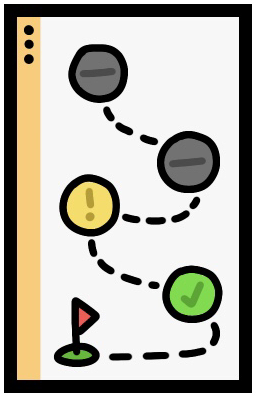
\includegraphics[width=\textwidth]{MainScreen.png}\\
    		\caption{Main Screen}
    	\end{subfigure}
    	\hspace{1em}
    	\begin{subfigure}[b]{0.203\linewidth}
    		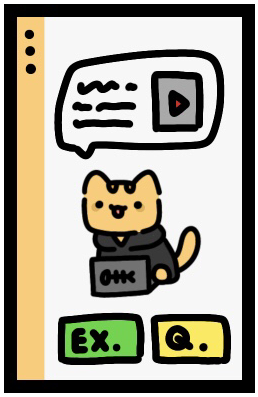
\includegraphics[width=\textwidth]{Lecture.png}\\
    		\caption{Lesson Screen}
    	\end{subfigure}
    	\caption{Example designs of the UI}
    	\label{fig:UI Ex}
    \end{figure}
    
\newpage

In main screen, 3 types of buttons can be seen in the middle of the screen. These are the mastered lesson, on-going lesson, and locked lesson. The green button represents the mastered lesson, means that the learner have already gotten a good grip on the selected topic. To get this button, learner must have already passed the quiz of the lesson. The yellow button represent the on-going lesson. The topics with this button as its representation are topics that learners have unlocked and started the lecture part. The gray button means that the lesson is locked and thus learners cannot go into those lessons. To change the gray button into a yellow one, learners must pass the quiz of the current on-going lesson first.

In the lesson screen, learners can see 3 things: the thumbnail of the lecture for the topic, button to the exercises (the green button), and the button to the quiz of the lesson (the yellow button). In here, learners can press the thumbnail to play the recorded lecture before doing the exercises, start doing the exercises, or head straight to the quiz button to skip the current lesson and move on to the next one. The answers from the exercises in the green button will be collected to evaluate the learner's skill and adjust the difficulty if needed (from easy to medium to difficult).
    
\newpage

\section{Game Design}
Types of exercises that will be integrated into the game are detect the error, code blocking, and fill in the blank (both via typing and drag-\&-drop). The examples of the exercise design is shown below in Figure 3.2. The lesson will be a mixed type where the user is introduced with the lecture and be led into the exercise part to help them understand and master their programming skill.There also would be interaction exercises in lecture where the mistakes here will not be counted towards the review calculation and the examples used will be easy for users to understand the basic concept.
	\begin{figure}[!htbp]
		\centering
		\begin{subfigure}[b]{0.2\linewidth}
			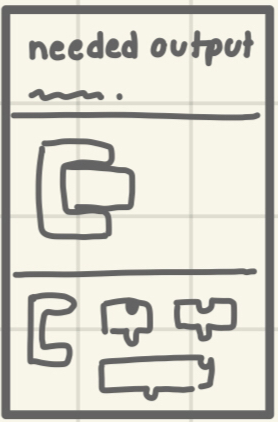
\includegraphics[width=\textwidth]{Ex3.png}\\
			\caption{Block Coding}
		\end{subfigure}
		\hspace{1em}
		\begin{subfigure}[b]{0.2\linewidth}
			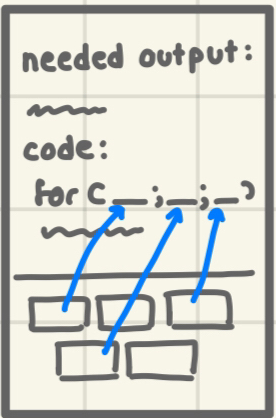
\includegraphics[width=\textwidth]{Ex1.png}\\
			\caption{Drag \& Drop}
		\end{subfigure}
		\hspace{1em}
		\begin{subfigure}[b]{0.2\linewidth}
			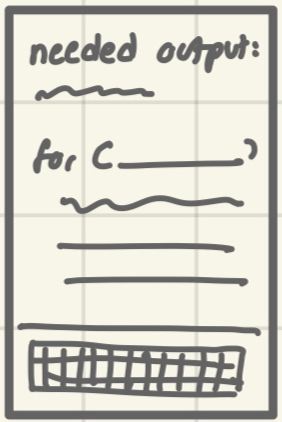
\includegraphics[width=\textwidth]{Ex2.png}\\
			\caption{Line Coding}
		\end{subfigure}
		\hspace{1em}
		\begin{subfigure}[b]{0.2\linewidth}
			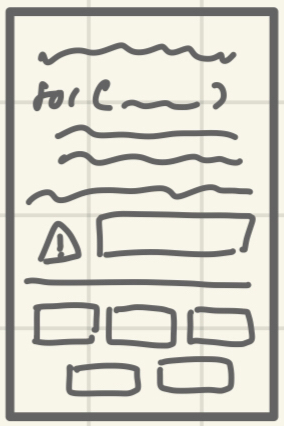
\includegraphics[width=\textwidth]{Ex4.png}\\
			\caption{Error Detect}
		\end{subfigure}
		\caption{Example designs of the lessons and exercises}
		\label{fig:Exercises}
	\end{figure}
	
\newpage

The block coding is usually in the beginning of the game to help the learners adjust to the way of programming by giving the learners the clear visual demonstration on how the code works. Learners will connect the given blocks in order to be able to produce the given output that the questions wants.

The drag \& drop can be seen as a transition phase from block coding to line coding. The way this works is that users will still be performing in a similar way as previous exercise where learners just drag the block around. The code of the question will look more like the line coding, but the way learners will approach the exercise will be similar to the block coding. Learners will be given keywords and they will have to put in the correct one in the correct place.

The line coding is the typical coding exercise where the learners will have to write a program from scratch and have the code run and output the needed output with the correct method if instructed.

The error detection exercise is another type of exercises in the application where the learners will have to identify the area where the code got its error message. After finding out the site of error, learners will have to rewrite the error part, so that the code can run and give needed output properly again.

\section{Evaluation Method}
The evaluation method will be divided into 2 categories : the first category is to evaluate learners if they can learn and understand more with aid of the application by knowledge checking learners with pre-test \& post-test in which the test will be separate into 2 sections. 

The first section will be the topics that students have already learned from the class and the other section will be topics that student haven't studied in the class yet. 

The second category of our evaluation is the engagement which we will be evaluating by using the evaluation form, login streaks, accumulate time spent playing the game, etc.